%\documentclass[times, 10pt, twocolumn]{article} 
%\documentclass[conference,final]{IEEEtran}
     
\documentclass{rspublic}   

%\usepackage{latex8}
%\usepackage{times}

%\documentstyle[times,art10,twocolumn,latex8]{article}

%------------------------------------------------------------------------- 
% take the % away on next line to produce the final camera-ready version 
%\pagestyle{empty}

\usepackage[utf8]{inputenc}
\usepackage{graphicx}
\usepackage{url}
\usepackage{float}
\usepackage{times}    
\usepackage{multirow}    
\usepackage{listings}   
\usepackage{times}     
\usepackage{paralist}    
\usepackage{wrapfig}    
\usepackage[small,it]{caption}
\usepackage{multirow}
\usepackage{ifpdf}    
\usepackage{subfig} 
                    
%Bibliography                     
\usepackage{natbib}   

\usepackage{listings}
\usepackage{keyval}  
\usepackage{color}
\definecolor{listinggray}{gray}{0.95}
\definecolor{darkgray}{gray}{0.7}
\definecolor{commentgreen}{rgb}{0, 0.4, 0}
\definecolor{darkblue}{rgb}{0, 0, 0.4}
\definecolor{middleblue}{rgb}{0, 0, 0.7}
\definecolor{darkred}{rgb}{0.4, 0, 0}
\definecolor{brown}{rgb}{0.5, 0.5, 0}

\lstdefinestyle{myListing}{
  frame=single,   
  backgroundcolor=\color{listinggray},  
  %float=t,
  language=C,       
  basicstyle=\ttfamily \footnotesize,
  breakautoindent=true,
  breaklines=true
  tabsize=2,
  captionpos=b,  
  aboveskip=0em,
  %numbers=left, 
  %numberstyle=\tiny
}      

\lstdefinestyle{myPythonListing}{
  frame=single,   
  backgroundcolor=\color{listinggray},  
  %float=t,
  language=Python,       
  basicstyle=\ttfamily \footnotesize,
  breakautoindent=true,
  breaklines=true
  tabsize=2,
  captionpos=b,  
  %numbers=left, 
  %numberstyle=\tiny
}


\title[Adaptive Distributed Replica-Exchange Simulations]{Adaptive Distributed
  Replica-Exchange Simulations}

% \title[Distributed Replica-Exchange Simulations]{ Distributed
%   Replica-Exchange Simulations on Production Environments using SAGA
%   and Migol}

% \title{Reliable Replica-Exchange Simulations of Biomolecular Systems
%   on Production Distributed Environments using SAGA-CPR and Migol}
% Computational Grids using SAGA-CPR and Migol}


\author[Luckow, Jha, Kim, Merzky, Schnor]{
  Andr\'e Luckow$^{1}$, Shantenu Jha$^{2,3,4}$, Joohyun Kim$^{2}$, Andre Merzky$^{2}$ and Bettina Schnor$^{1}$\\
  \small{\emph{$^{1}$Institute of Computer Science, Potsdam University, Germany}}\\
  \small{\emph{$^{2}$Center for Computation \& Technology, Louisiana State University, USA}}\\
  \small{\emph{$^{3}$Department of Computer Science, Louisiana State
      University, USA}}\\
  \small{\emph{$^{4}$e-Science Institute, Edinburgh, UK}}\\
}

%\date{}

\def\acknowledgementname{Acknowledgements}
\newenvironment{acknowledgement}%
{\section*{\acknowledgementname}%
\parindent=0pt%
}

\newif\ifdraft
% \drafttrue
\ifdraft
\newcommand{\kimnote}[1]{ {\textcolor{green} { ***JK: #1 }}}
\newcommand{\alnote}[1]{ {\textcolor{blue} { ***AL: #1 }}}
\newcommand{\amnote}[1]{ {\textcolor{magenta} { ***AM: #1 }}}
\newcommand{\jhanote}[1]{ {\textcolor{red} { ***SJ: #1 }}}
\else
\newcommand{\kimnote}[1]{}
\newcommand{\alnote}[1]{}
\newcommand{\amnote}[1]{}
\newcommand{\jhanote}[1]{}
\fi

\newcommand{\glidein}[1]{Glide-In }  
\newcommand{\replicaagent}[1]{Replica-Agent }         
\newcommand{\remanager}[1]{RE-Manager }

\begin{document} 


\maketitle    

\begin{abstract}{Replica-Exchange, SAGA, Migol, Fault Tolerance}  
  % There exists a class of scientific applications for which
  % utilizing distributed resources is critical for reducing the
  % time-to-solution. However, try to avoid redundancy within the
  % abstract - BS

%   One challenge arises from the need to orchestrate many tasks over
%   multiple resources; another arises from the desire to create an
%   infrastructure independent approach.
%   is helpful, if not critical for the effective solution of the
%   scientific problem.

  The ability to effectively utilise multiple distributed resources to
  reduce the time-to-completion remains a challenge at many levels.
  We discuss the Replica-Exchange (RE) class of applications, which in
  principle, due to the loose-coupling of the sub-tasks (replicas),
  can benefit greatly from utilising as many resources as available --
  distributed or otherwise.  An implementation of a {\it
    pleasingly-distributed} algorithm like RE that is
  independent of infrastructural details however does not exist.  This
  paper proposes an extensible and scalable framework based on SAGA
  and Migol that provides a general-purpose, opportunistic mechanism
  to effectively utilise multiple resources in an infrastructure
  independent way. By analysing the requirements of the RE algorithm
  and the challenges of implementing it on real production systems, we
  propose a new abstraction (BigJob), which forms the basis of the
  adaptive redistribution of replicas and the effective scheduling of
  the multiple sub-tasks.
  
  \jhanote{AndreL: I changed resources in the last sentence to
    replicas. Let me know if you agree?}

  \jhanote{Just as a general remark, if we have adaptive in the title,
    it is only proper that we also have the word ``Adaptive'' in the
    abstract}

  % Looks like buzzword parade to the reader - I prefer to skip it The
  % implementation of our framework can be used in clusters and Grid
  % supporting single-processor as well as multi-processor simulations
  % that require tightly-coupled resources.

  % SAGA is a high-level programmatic abstraction layer that provides
  % a standardised interface for the distributed functionality
  % required for application development. Migol provides the
  % underlying middleware which ensures the reliable execution of
  % applications even in the presence of failures.

 % SAGA~\citep{saga_gfd90} and Migol~\citep{schnorLuckow08} for

  \jhanote{In this paper, we describe the design, development and
    deployment of a unique framework for constructing fault-tolerant
    distributed simulations.}

  \jhanote{Less emphasis on the SAGA/Migol framework: The framework
    consists of two primary components -- SAGA and Migol, is scalable,
    general purpose and extensible.}

  \jhanote{I think this can go: We provide details of a newly
    developed functionality in SAGA -- the Checkpoint and Recovery
    API. Migol is an adaptive Grid middleware, which addresses the
    fault tolerance of Grid applications and services by providing the
    capability to recover applications from checkpoint files
    transparently.  In addition to describing the integration of
    SAGA-CPR with the Migol infrastructure,} \alnote{I added a small
    note about Migol to the abstract (I tried to keep it short.)}

  \jhanote{We also outline our experiences with running a large scale,
    general-purpose, SAGA-CPR based RE application in a
    production distributed environment.}

\end{abstract}

\section{Introduction}

\jhanote{General Remark: Replica-Exchange is used as i) application
  class, ii) algorithm, and iii) simulations. We'll need to be
  careful. Fundamentally it is a class-of-algorithms, one which
  applications are based and simulations of which are carried out!}

\jhanote{General Remark: We are using RE and Replica-Exchange interchangeably?
  In principle, once we've defined RE (I think in Section 1 itself), we 
  should just use RE and not Replica-Exchange. AndreL: Can you make this
  consistent please?}
\alnote{Ok. RE is consistently used (except in captions)}

\jhanote{Need to add what is the unique contribution of this work? How
  it extends earlier work and forms the basis of future work.. (maybe
  this goes into the conclusion section)}

%%%%% problem setting: pleasingly distributed RE
Several classes of applications are well suited for distributed
environments. Probably the best known and most powerful examples are
those that involve an ensemble of decoupled tasks, such as simple
parameter sweep applications. \jhanote{Can we put a simple reference
  here? Either to a famous parameter sweep study, or to a system such
  as APST that supports parameter studies} A slightly more complicated
and challenging class of distributed applications are those that have
a degree of coupling between individual sub-tasks.  An interesting
example of such applications are those based upon the
\emph{Replica-Exchange (RE)}~\citep{hansmann,Sugita:1999rm}
algorithm. \jhanote{Was simulation before algorithm... We were making
  sloppy errors here.. for example equating applications and
  simulations!} RE simulations are e.\,g.\ used to understand
important physical phenomena -- ranging from protein folding dynamics
to binding affinity calculations required for computational drug
discovery.
  
%%%%% RE nature of the problem
RE simulations involve the concurrent execution of multiple
simulations -- the \emph{replicas}. The coupling between replicas
takes place in the form of periodic exchange attempts between paired
replicas. Typically coupling occurs infrequently compared to the
run-time of each replica and is small in terms of communication
bandwidth requirements; thus RE is {\it prima facie} a perfect
algorithm to exploit distributed resources. We label such a class of
algorithms as {\it pleasingly-distributed}.

% Despite their essentially loosely-coupled nature, RE simulations
% require a level of coupling: the coupling is in the form of exchanges
% that occurs infrequently compared to the run-time between exchanges,
% and it is small in that the communication bandwidth requirement is
% small.  Thus, RE is {\it prima facie} a perfect algorithm to exploit
% heterogenous, loosely-coupled distributed resources.

%%%%% related work
Most RE implementations are either infrastructure
specific~\citep{Woods:2005nx}, or require prior co-scheduling of
distributed resources~\citep{repex_mpig}.  
% Work reported in Ref[~\citep{repex_mpig}] 
In particular, the work reported by~\citet{repex_mpig} is an important
example of first-generation Grid applications, wherein the
effectiveness of coupling multiple distributed resources for
scientific problems has been demonstrated.  \jhanote{AndreL, I know we
  are short on space, but the above line is politically important and
  will help smoothen the passage of this paper} The real power of
distributed systems however, arises from adaptive algorithms and
implementations that provide applications with an agile execution
model, and thus the ability to utilise resources dynamically, as
opposed to a static execution model inherited from parallel and
cluster computing.  Unfortunately, the barrier to the development of
such adaptive applications is high and the infrastructure support for
applications with dynamic resource utilisation requirements poor.
Therefore, it is not surprisingly that there do not exist more
adaptive applications in general, but specifically there does not
exist an implementation of an adaptive RE algorithm, which is both
able to effectively and reliably utilise multiple distributed
resources without prior scheduling as well as being independent of any
specific computational platform or infrastructure.
                      
%%%%% reference to contribution of escience paper
To address heterogeneity and failures, which are both inherent
characteristics of distributed systems, we demonstrated the use of
SAGA~\citep{saga_gfd90}, in particular its Checkpoint Recovery (CPR)
package, and of the Migol middleware~\citep{schnorLuckow08} to build a
reliable RE application~\citep{Luckow:2008la}.
% Further, we showed its usability on several different resources.
In general, SAGA and Migol provide the tools for developing a broad
range of reliable applications, of which RE is a specific example.
% of a loosely-coupled application. 
Implementing a framework with the ability to handle faults and
heterogeneity, was an important first-step on the critical-path
towards developing a framework that can support adaptive RE simulations on
production-level infrastructures.

%%%%% contributions of this paper  
%%%%% SJ original below
This paper arises from practical considerations related to the
deployment of a distributed, loosely-coupled application.  We address
some of the challenges and performance bottlenecks encountered when
using the framework \jhanote{I'm not convinced the reader knows what
  ``the framework'' at this stage means. Are you?} in a production
environment %A major concern that arises for example, is the overall
such as the overall slowdown due to synchronisation arising from the
light-coupling and the lack of co-scheduled resources. Production
distributed environments in their current incarnation are manifest as
an aggregation of multiple single-resources. Although there are some
initial attempts at supporting co-scheduled resources for
tightly-coupled simulations~\citep{repex_mpig}, there are insufficient
attempts at supporting a broader range of distributed and collective
modes of operations, such as required for loosely-coupled
applications.  For example, current infrastructure does not provide
efficient {\it application-level} mechanisms for co-ordinated resource
sharing. One approach to rectify these deficits are system-level
abstractions that allow applications to effectively utilise
distributed resources concurrently.

The unique contribution of this paper is the implementation of RE
framework that overcomes the described limitations, by being able to
adapt at runtime to a change in the resource availability and
application resource requirements. The framework utilises the
\emph{BigJob} abstraction, \jhanote{Andre L please let me know if you
  agree with this addition? -- ``in combination with the Glide-In
  mechanism''} which in combination with the Glide-In mechanism,
allows the efficient dispatching of jobs by grouping smaller sub-jobs
% utilisation of distributed resources without prior co-scheduling 
into a larger job. \jhanote{I'm wondering if we should call BigJob
  novel or is the framework that is
  novel?}  
\alnote{I would call the abstraction novel. As we learned today there
are a couple of Glide-In frameworks out there.} 
% The BigJob abstraction also serves as basis for
% supporting adaptive RE simulations.
\jhanote{Also in the previous sentence, I agree with the first part --
  ``bigjob allows the utilisation of distributed resources without
  prior scheduling'', but dont agree with the latter part of the
  sentence, ie this is achieved by grouping smaller-jobs into a larger
  job. this bit allows the individual jobs to be efficiently
  scheduled, not distributed utilisation. Does this make sense?}
\jhanote{Remember this is a paragraph in the opening/introduction
  section, hence will be scrutinised more carefully} \alnote{Agree, I
  dropped the co-scheduling stuff from the sentence before, since the
  remainder of the paragraph focuses on adaptiveness.}  The RE
framework relies on the \emph{BigJob} abstraction not only for
dispatching replica jobs, but also adds higher-level functionality by
allowing the dynamic utilisation of additional resources as they
become available.  Our implementation is both independent of the
platform and infrastructure details, and can respond gracefully to
failures.  We present data that validates the claim that as more
resources become available our framework can opportunistically employ
these resources to lead to a reduction in the time-to-completion of
the scientific problem.  Although the tests we report here are still
experiments (i.e., we are not reporting science results in this
paper), it is critical to note, that these are done on production
infrastructure such as the TeraGrid under exact conditions encountered
by application-scientists and not on research infrastructure such as
Grid5000\jhanote{suitable reference here please}.


%%%%%%%%%%%%%  Shantenu original %%%%%%%%%%%%%                                                  
% The heterogeneity and dynamism of a computational Grid results in
% increased difficulty and complexity in developing and deploying
% adaptive, distributed applications.  
% To master this complexity, a well-defined programming abstraction as 
% well as a sophisticated middleware is required. 
% The abstraction should allow scientists to
% focus on the application logic, while the middleware provides critical
% services, such as reliable job management and monitoring.
% However, abstractions that enable effective distributed application development,
% are not sufficient.  Distributed applications need to operate 
% and execute in real production environments; 
% however, production distributed environments are in
% their current implementation and incarnation up to now, the aggregation
% of multiple single-resources and there are no explicit attempts at
% supporting the collective, distributed mode of operations.  For
% example, production infrastructure does not provide a mechanism for
% co-ordinated resource sharing; one approach to rectify this deficit is
% via system-level abstractions from which such higher-level
% functionality can be provided.

% Some applications can respond to such failures via redundant or
% speculative computing.  However, redundant computing has its
% limitations, especially when there is a level of heterogeneity and
% coupling between tasks.  Speculative computing is still possible, but
% its use to mitigate the consequence of distributed failures, leads to
% a whole host of load-balancing and scheduling problems.  
        
% \jhanote{Need to consider this paragraph a bit more carefully. Could
%   go against us.}         

% The unique contribution of this paper is the implementation of a
% framework that enables the effective collective utilisation of
% multiple distributed resources that overcomes production-grade
% infrastructure limitations without prior co-scheduling. 
% Our implementation is both independent
% of the platform and infrastructure details, and can respond gracefully
% to fault-tolerance.  We present preliminary data that validates the
% claim that as more resources become available our framework can
% opportunistically employ these resources to lead to a reduction in
% the time-to-completion of the scientific problem.    

The remainder of the paper is structured as follows: In the next
section we provide the basic ideas behind RE and specifically
RE using Molecular Dynamics (REMD) simulations.  We then
briefly discuss the SAGA/Migol fault-tolerant framework in
section~\ref{sec:sagamigol}.  In section~\ref{sec:remd_impl}, we
describe the details of a REMD application implemented using the
SAGA/Mi\-gol framework. Section~\ref{sec:glidein} discusses the new
BigJob abstraction and the SAGA Glide-In framework.  We highlight
different adaptivity strategies for supporting dynamic applications in
section~\ref{sec:adaptivitiy}.  In the subsequent section we discuss
the deployment and results of experiments using the SAGA based
RE framework on the TeraGrid.  We conclude by discussing
related work -- which will highlight the unique features
of our implementation, and provide a glimpse of future work
in this direction.

\jhanote{AndreL: if we don't provide a mention of future work at the
  end, please highlight: i) the use of intelligent placement ii)
  using this to solve real Riboswitch problem. Use this citation
  please: Huang, Wei; Aboul-ela, Fareed; Jha, Shantenu; Boyapati,
  Vamsi. Computational study of conformational switching of s-box
  riboswitch. Poster at 235th ACS National Meeting, New Orleans, LA,
  United States, April 6-10, 2008 (2008), BIOL-182. at
  http://www.cct.lsu.edu/~whuang/}       
\alnote{added}

\ifdraft \alnote{I moved the itemize to the draft mode. We probably
  still need to add some of these points to the text above.}

\jhanote{I would like to put this into the document here, but the
  introduction is already long ~2pages, plus I don't want to have this
  be an indirect criticism of tightly-coupled applications on Grids,
  which I'm no fan of, but this is not the place/journal to make that
  argument!}

\begin{itemize}
  \item The move of traditional algorithms to distributed systems holds
    the promise of reduced time-to-solution and other advantages, but
    comes with its own set of challenges. For example, there is a
    trading of control and comfort of a single environment, for the
    coordination hassles of distributed systems. In particular, the need
    to schedule multiple resources is challenging. The stringency of the
    requirement of scheduling resources changes with the level of
    application-level coupling. For example, for tightly-coupled
    MPICH-G2 style jobs, complete synchrony is required; for
    loosely-coupled applications/replicas there is still a need to
    co-schedule resources, but the choice of clever
    algorithms/implementations can relax this requirement. In
    pathological cases, all systems can come to a grinding halt if a
    global synchronization of the different components is required
    between successive stages, and any one component has not even
    started!  

    \alnote{What is category RE simulations fall into according to the
      DPA categorization: pleasingly distributed, loosely coupled with
      homogeneous sub-tasks, loosely coupling of tightly-coupled
      applications? All?}
  
    \jhanote{RE are loosely-coupled simulations with homogenous
      sub-tasks. Depending upon specific simulations undertaken it can
      also be loose-coupling of tightly-coupled applications}

    \alnote{Do we really deliver the promise of a clever algorithm
      yet? Or are we promising here to much? Maybe we should separate
      application algorithm and efficient scheduling which is more a
      infrastructure capability?}

    \jhanote{There are multiple physical algorithms that can be
      used to solve the same physics problem (more-or-less).
      However, the choice of which one of those to use can be
      clever (decomposable, loosley-coupled) or foolish (monolithic
      and long running). Make sense?}

  \item There are different levels of abstractions that are required
    in order to make distributed systems generally more usable for
    production science. By one classification, the three levels are,
    i) application level, ii) deployment iii) system-level level
    (usage) abstraction.


    \alnote{Mostly relevant for this paper should be only system-level
      abstractions. Thus, I am not sure whether we should address all
      types of abstraction}

   \jhanote{Application == SAGA; BigJob == deployment; GlideIn ==
      System (those with schedulers). Hence I claim all three levels
      are covered here.}

  \item A unique/novel contribution of this paper is the first
    implementation of a system-level abstraction (inspired by the
    Condor Glide-In mechanism~\citep{citeulike:291860}) using
    programmatic interfaces, and a novel implementation of the
    RE algorithm to exploit resources opportunistically.
    However it is critical to point out that the {\it novel} RE
    implementation is practical only because of {\bf the agile
      execution model} that the programming model and system provide.
    The generalization of the RE algorithm is conceptually simple, but
    ensuring its implementation and deployment is not, and {\bf
      depends critically upon support for the nimble execution
      provided by SAGA's enhanced job model and the system-level
      abstractions}

  \item The developed application framework is able to dynamically
    adjust the scope of the simulation according to the currently
    available resources.

  % \item Algorithmic behaviour/constraints on a localized/single cluster
  %   can be very different for distributed clusters. Interesting to
  %   mention that it is trivial to port this framework onto a top-end
  %   machine such as Ranger that is pushing the limits of petascalabilty.
\end{itemize}
\fi

\section{Replica-Exchange Molecular Dynamics}
\alnote{I restructured this section: 1) general introduction to MD
  problems and further motivation for RE algorithm 2)
  Structure/Classification of REMD algorithms}  In Molecular
Dynamics (MD) approaches, a sufficient sampling of configurations is
an important requirement for connecting atomistic results to
macroscopic or thermodynamic quantities available from experiments.
However, even with the most powerful computing resources at the
moment, straight-forward MD simulations are unable to reach the
relevant time-scales required to study conformational changes and
searches. This is partly due to the inherent limitations in the MD
algorithm -- a global synchronization is required at the end of each
time step.  This provides an important motivation for research into
finding ways to accelerate sampling and enhance ``effective''
time-scales studied. Generalized ensemble approaches -- of which
Replica-Exchange Molecular Dynamics (REMD)~\citep{Sugita:1999rm} are a
prominent example -- represent an important and promising attempt to
overcome the general limitations of insufficient time-scales, as well
as specific limitations of inadequate conformational sampling arising
from kinetic trappings.  The fact that one single long-running
simulation can be substituted for an ensemble of shorter-running
simulations, make these ideal candidates for distributed environments.

RE simulations can be thought of as consisting of
two distinct components: the underlying simulation engine/mechanism
used for each replica, and the coupling-mechanism between the
individual replicas.  It is important to note that RE is in fact a
class of algorithms and not a specific
algorithm~\citep{dpa-paper}; for example, there can be not only
different simulation strategies -- such as the Monte Carlo and the
described MD approach -- but also multiple levels-of-coupling.  

The degree and frequency of coupling and exchange can be either
regular~\citep{hansmann,Sugita:1999rm}, or
irregular~\citep{SPdynamics,pande_bj03}. An example of the latter --
parallel replica dynamics as implemented in Folding@home
\citep{folding} involves coordination between replicas only when an
``event'' occurs.  In contrast, for regular RE applications, attempts
to exchange states between certain pairs occur at fixed intervals. A
major challenge common to both types however, is the design,
development and deployment of a general purpose RE framework for
distributed environments.



\section{SAGA/Migol: Providing a Fault-Tolerant Framework 
for Replica-Exchange Simulations}\label{sec:sagamigol}

% Fault Tolerance
\jhanote{I think we need just a paragraph or two at most, outlining
  what SAGA Migol does and why it is required critically for the
  replica exchange applications. Reference the IEEE e-Science paper
  and say that details of the integration of SAGA-Migol are presented
  there.}

% Distributed computing environments are inherently prone to 
% failures~\citep{schroeder,10.1109/E-SCIENCE.2006.93,DBLP:conf/grid/KhaliliHOSC06}. 
% The more resources involved, the greater the probability of a failure.
% Replica-Exchange simulations are very fragile: the loss of a single
% replica process due to a node or network failure usually causes the
% abort of the entire simulation. Thus, the middleware must detect and
% resolve failures, such as the crash of the Globus GRAM or of a
% resource running parts of the RE application, accurately.

The framework used for implementing REMD consists of two primary
components: the \textit{Simple API for Grid Applications
(SAGA)}~\citep{saga_gfd90} and Migol~\citep{schnorLuckow08}.  While
SAGA represents a well-defined, standardized abstraction for writing
Grid applications, Migol provides the underlying middleware services
to guarantee the correct and reliable exe\-cution of applications even
in the presence of failures.

Distributed systems are inherently prone to 
failures~\citep{schroeder,10.1109/E-SCIENCE.2006.93}.    
In particular, RE simulations are very fragile: the loss of a single
replica due to a node or network failure usually causes the
abort of the entire simulation. Migol is an adaptive Grid middleware 
that provides several mechanisms for supporting the fault tolerance of 
distributed applications. 
The framework can automatically detect and transparently handle common
failures, such as node or application crashes. For recovery Migol
relies on application-level checkpointing to ensure that the amount of
lost computation is minimized. The application is solely responsible
for registering job and checkpoint metadata with the central registry
service of Migol. Once registered, Migol will handle the monitoring
and, if necessary, the recovering of the application.

% The framework is based on the Globus Toolkit 4.  

The SAGA CPR API provides a high-level programming abstraction for
starting, monitoring and recovering of checkpoint-restartable jobs. To
support these use cases, applications can register checkpoint and job
metadata with a Grid middleware, such as Migol, using this API.
% Migol represents the natural counterpart for the SAGA CPR API. 
Migol has been seamlessly integrated into the SAGA C++ reference
implementation~\citep{Kaiser:2006qp} using the provided adaptor
mechanism. Details of the SAGA/Migol integration are described
in~\citet{Luckow:2008la}.

SAGA and Migol offer a scalable, general purpose and extensible
environment for developing resilient Grid applications.  Using a
powerful abstraction, such as SAGA CPR, applications can easily and
reliable orchestrate hundreds of checkpoint-restartable tasks and
benefit from an adaptive infrastructure such as Migol at the same
time.

\jhanote{Are we using SAGA-CPR Migol here for checkpointing? or
  error/fault detection} 
\alnote{We support SAGA-CPR/Migol in the code... No experiments done though}  

\alnote{Almost all of this issues are mentioned in the introductions,
  I am therefore not sure whether we still need this section?
  Shantenu, what do you think}

\jhanote{I've kind of reduced mention/details of SAGA/Migol in the
  introduction (so as to focus on the new stuff), so its OK here now,
  I think}

% Programming abstraction Implementing a RE application that is
% capable of running in a heterogeneous and distributed environment is
% a complex task. RE simulations involve the parallel orchestration of
% many replica jobs. To master this complexity, a well-defined
% programming abstraction as well as a sophisticated middleware is
% required. The abstraction should allow scientists to focus on the
% application logic, while the middleware provides critical services,
% such as reliable job management and monitoring.
% 
% % Synchronization & Scheduling issues
% Despite their mostly loosely coupled nature, RE simulations require
% a small level of coupling.  The central master, the RE-Manager, must
% periodically obtain the results, i.\,e.\ the energy levels, of all
% replicas to determine the new configuration of the next RE step.  
% This significantly limits the applicability of RE to heterogenous 
% distributed environments, such as Grids.  Even on a single machine 
% the required synchronization leads
% to various load-balancing and scheduling issues. In distributed
% environments jobs often experience large slowdowns due to
% long queueing times in particular when using production resources. 
% Such delays can have a severe impact on the overall time to
% completion.                                                    
% In our earlier experiments~\citep{Luckow:2008la} this obstacle  
% became evident -- for individual RE runs on a single machine, 
% as well as for runs across different heterogeneous resources.
% Especially when running replicas across multiple resources, 
% a single crowded resource can delay the completion of the 
% simulation arbitrary. Thus, an efficient mechanism for dispatching 
% sub-jobs across multiple distributed resources
% is required.
%                  
% % Fault Tolerance
% Another important issue in error-prone distributed environments is
% fault tolerance.  Especially RE simulations are very fragile: the
% loss of a single replica due to a node or network failure
% usually causes the abort of the entire simulation. Thus, the
% middleware must detect and resolve failures, such as the crash of the 
% Globus GRAM or of a resource running parts of the RE application, accurately.
%                                   
% % not synthetic, real and meanginful physical models 
% \alnote{I am not sure whether we keep this claim... - maybe we should not promise
% too much...}
% Implementing an approach that can scale up to very large 
% production infrastructures is a far more challenging task than
% implementing a toy-model on a research environment. Our approach is
% aimed strictly at the former, to provide a basis for real scientific
% problems. The scale-up and complexity of production environment makes
% this extension non-trivial.     

% Another challenge in a heterogeneous environments is the
% synchronization required after each round. In particular, when
% running RE across multiple clusters the effects of queue wait
% times can be severe. To avoid this issue, a middleware must provide
% efficient mechanisms to allocate resources for multiple replica runs
% in a row.

\alnote{The scheduling and reliability sections partially already described the solution. 
I added the important points to challenges. The description of our approach have been 
moved back to the Implementation and Scheduling section.}
                         
\section{Implementing Distributed Replica-Exchange Using SAGA/Migol}
\label{sec:remd_impl}
\jhanote{this is an important section. we need to put in details of
  how our implementation addresses issues of bigjob/smalljob to
  overcome restarting one one machine and how we overcome slowdown due
  to different scheduler loads on different machines..}

% The \emph{Simple API for Grid Applications (SAGA)}~\citep{saga_gfd90}
% provides an easy-to-use, standardised API for developing a broad range
% of distributed applications, including, but not limited to
% loosely-coupled applications.  In particular, SAGA CPR and Migol allows 
% the efficient management of checkpoint-recoverable jobs. 
% Thus, SAGA is ideally suited for
% encoding the orchestration logic of RE simulations.      

This section outlines the architecture and implementation of the RE
framework using SAGA and Migol.

\jhanote{Put in a paragraph or two of the main points of the
  how it is done here; maybe even discussing the ideas related to
  checkpointing, new jobs, MPI issues discussed etc. etc. Try to
  establish what is specific to the SAGA way of doing things from what
  is a general distributed computing problem/issue}

\jhanote{I still think that at some stage -- maybe not in this paper,
  the above point should be addressed}      
  
\alnote{I added a paragraph highlighting the SAGA way (decoupling, transparent use of migol).}  
          
\subsection{RE-Manager Architecture}

\begin{figure}[t]
      \centering
          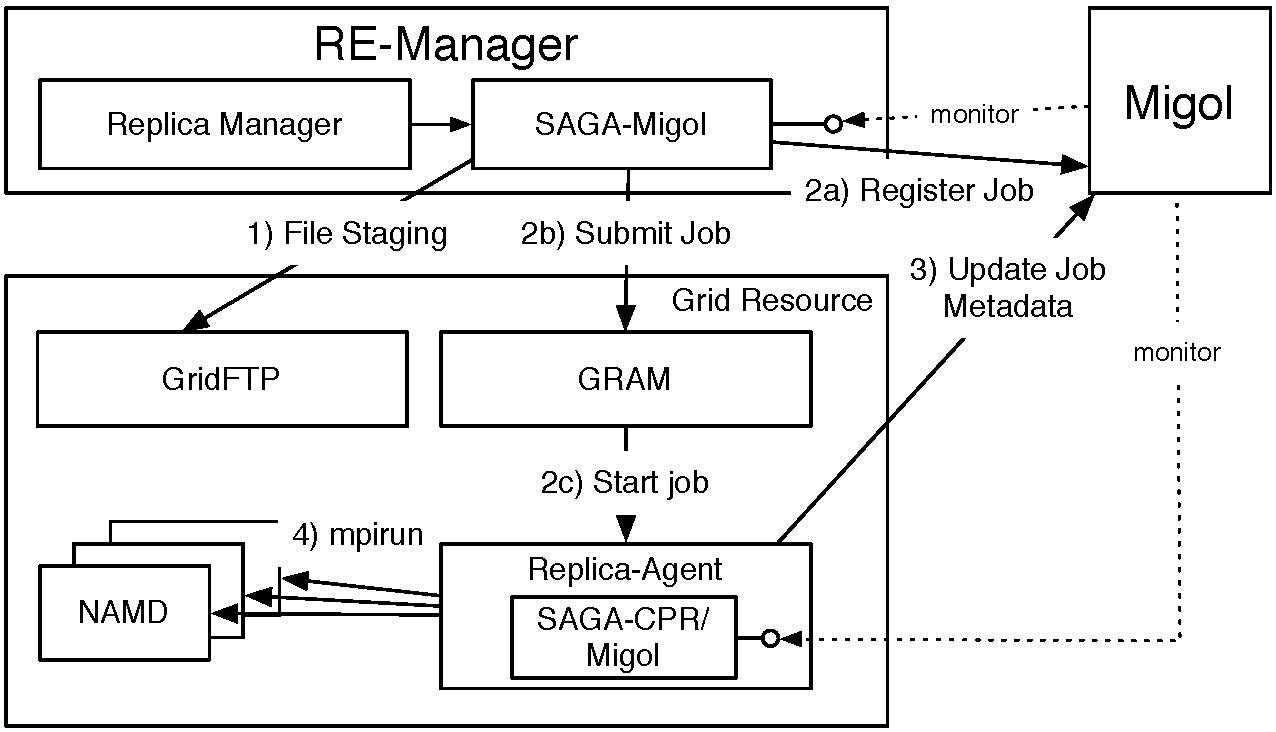
\includegraphics[width=0.8\textwidth]{REMDgManager-architecture.pdf}
          \caption{\footnotesize \bf RE-Manager Architecture: The
            core of the framework, the RE-manager, orchestrates 
            a set of distributed replicas using SAGA \& Migol. 
            The Replica-Agent is responsible for managing and monitoring 
            replicas on a single machine. Finally, the Migol 
            infrastructure ensures that the RE-Manager and the Replica-Agent 
            are monitored and recovered if necessary.            
            \jhanote{The caption of this
              figure need to changed to be in harmony with the opening
              paragraph of ``RE-Manager Architecture'', where this
              figure is referenced and discussed. I.e., we talk about
              three components in that paragraph, this caption should
              be structured accordingly too.}
              \alnote{Reworked caption to highlight this three components. 
              I am not sure whether this is a good time to introduce the GlideIn stuff. But, I 
              decided to leave this for the next subsection to focus initially on
              the efficient implementation of RE}
              }
      \label{fig:REMD-Manager-architecture}
\end{figure}

As illustrated in Figure~\ref{fig:REMD-Manager-architecture}, the
proposed framework comprises of three components, the RE-Manager,
the Replica-Agent and the Migol infrastructure. 
The  \emph{RE-Manager}, also referred to as task manager,
is deployed on the user's desktop and provides the user interface 
to the overall RE run. It orchestrates all replicas, i.\,e.\ the 
parameterization of replica  tasks, file staging, job spawning 
and the conduction of the RE itself using the SAGA CPR
and File API.                                                                

The second element is the task agent, the \textit{Replica-Agent},
that resides on the high performance machines where RE simulations
are carried out. The \replicaagent\ is launched using SAGA CPR and Migol.
It is responsible for spawning and monitoring of the replicas. 
NAMD~\citep{Phillips:2005gd}, a highly scalable, parallel MD
code, is used to carry out the MD simulation corresponding to each
replica run. It is important to mention that any other Molecular Dynamics 
or Monte Carlo code could be used just as simply and effectively.

The last component is Migol and the underlying Globus middleware. 
Migol handles the reliable execution of replicas, i.\,e.\ the submission,
the monitoring and, if required, the recovery of replicas or the application itself. 

In summary, SAGA allows the simple decoupling of the RE application 
logic from the underlying Grid middleware. It provides well-defined
abstractions for implementing the RE logic. At the same
time applications can benefit from Migol by simply configuring the corresponding
adaptor.


% The \emph{RE-Manager}~\footnote{The complete \remanager\ code can be found
% at https://svn.cct.lsu.edu/repos/saga-projects/applications/REMDgManager/}

% For the implementation 
% of the RE logic, this component heavily relies on the SAGA Python bindings 
% for accessing the File and CPR API as well as the enhanced job management 
% framework for efficient clustering of jobs. 
                                  
% \alnote{I am really not sure about this code snippet. It somehow
%   represents the logics - however I am not sure whether it is worth
%   the space.} \jhanote{I agree, that as written it is not very
%   effective. Also, since it does not show the exchange and thus the
%   reader does not see how ``distributed'' and ``local'' exchanges are
%   handled equally simply. Can we i) use psuedo-code to highlight this?
%   ii) mention where the reader can get the actually code?. We should
%   definitely do point ii) and possibly point i)}

\jhanote{This part currently conflates architecture and control-flow}
                       
\subsection{Replica-Exchange Logic}
                                            
RE simulations involve the running of multiple replica jobs to enhance the sampling. 
In the case of REMD each replica job is assigned a different temperature.  
Depending on the number of configured processes $n$, the \remanager\
creates $\frac{n}{2}$ pairs of replicas.
Before launching a job the \remanager\ ensures that all required input 
files are transfered to the respective resource. For this purpose, the SAGA File API and the
GridFTP adaptor (step 1 in Figure~\ref{fig:REMD-Manager-architecture})
are used.  The replica jobs are then submitted to the resource
using the CPR API and Migol/GRAM (step 2a-2c). Migol ensures that the
job description of each replica is stored within the Migol backend
to ensure a later recovery. Globus GRAM is used to start the
application.

When all replicas reach a pre-determined state (e.\,g., the NAMD job finishes 
after a fixed number of steps), the decision as to whether to pairwise 
exchange temperatures between neighbouring replicas
is determined by the Metropolis scheme~\citep{metropolis:1087}.    
A single exchange round, i.\,e.\ the run of an ensemble of
replicas in parallel and the subsequent attempt to pairwise
exchange, is referred to as generation.                                                         

If successful, parameters such as the temperature, are swapped. Both jobs are then
relaunched using the mechanisms described above. Often the Metropolis
scheme returns a negative result, and an exchange is not carried out;
thus it is difficult to respond to a possible exchange speculatively. 

\subsection{Reliability}
To achieve fault tolerance, the RE-Manager, the Replica-Agents and the
replicas periodically write persistent checkpoints to allow
an automatic recovery via the Migol infrastructure. The \remanager\
and Replica-Agents periodically update the application's metadata,
i.\,e.\ the state, monitoring endpoint and new checkpoint URLs, at the
Migol backend using the CPR API. During the entire runtime the
\remanager\ and the Replica-Agents are monitored by Migol using the
monitoring endpoint of the Replica-Agent. If a failure is discovered
by Migol, an automatic restart of an agent or the RE-Manager is
initiated.

\alnote{Should we make this a subsection or a section? In my opinion,
the GlideIn stuff is a major contribution of this paper -- thus I decided to
give it a separate section. I also think it is more readable than going to the
subsubsection level.}           

\subsection{Deploying on Production Environments: Scheduling}

The RE framework has been successfully deployed on
production environments, such as LONI and the 
TeraGrid~\citep{Luckow:2008la}. However, as the
number of replicas increase, the probability of an overall slowdown
caused by the synchronization required by the RE
algorithm after each generation increases.  The central master, the
RE-Manager, must periodically obtain the results of all replicas to
determine the new configuration of the next RE step. The replicas are
then re-started, i.\,e.\ they are required to queue again at the local
scheduler. In pathological cases, the complete system can come to a
halt caused by a single crowded or slow resource.  
                        
To avoid such bottlenecks, distributed applications must be able to 
respond to the dynamic availabilities of resources. This requires 
(i) sufficient system-level abstractions that enables an agile
execution model allowing an application-level allocation of resources, 
and (ii) different adaptivity strategies that determine how
resources are efficiently utilised. Unfortunately, current 
infrastructures lack both aspects. The following section 
describes different extensions to our RE framework that 
enable adaptive applications.



% which allows the simple clustering of tasks
\jhanote{Do you see the important difference: BigJob is the clustering
  of tasks; Glide-In is the scheduling mechanism that utilises it to
  solve the repetitive queuing problem}

\alnote{removed Glide-In introduction and move it to next
  section... Otherwise too much redundancy}
% Using the BigJob abstractions,
% applications can utilize this framework to implement different adaptivity
% strategies.

% We propose a novel, adaptive RE algorithm to relax this
% constraint. The adaptive RE algorithm permits a change in the number
% of replicas that are employed by adjusting the sampling range.  With
% this capability adaptive RE is able to opportunistically employ
% resources as they become available.
% The major cause for slowdowns are queueing delays, which particularly
% occur when using production resources. 

% To address this issue, we propose a ``Glide-In'' framework 
% based on SAGA (similar to Condor
% Glide-In~\citep{citeulike:291860}), which allows the direct
% dispatching of replica jobs and overcomes the need to co-schedule
% resources.  The enhanced job abstraction allows RE applications to
% efficiently cluster sub-tasks, which are executed on the same machine.
% The adaptive RE algorithm is build on top of this abstraction.
% Although the adaptive algorithm does not (and cannot) remove the need
% for synchronisation amongst the replicas at the exchange step, it
% ensures that a synchronization is only conducted between running
% replica processes on available resources, i.\,e.\ resources with an
% active Glide-In job.


% \section{SAGA Glide-In: Efficient Job Scheduling for Replica Jobs}
\section{Adaptive Replica-Exchange: Abstractions and Algorithms}
\label{sec:glidein}

As motivated before, the use of multiple {\it simple} Grid jobs to
execute many replicas has a severe limitation: all simple jobs must
queue at the resource management system. In this scenario, a single 
delayed job can cause the slowdown of the overall application. 
We overcome this issue by using an efficient dispatching scheme, 
which builds upon the ability to cluster replicas using the novel 
BigJob abstraction before submission. Based on this abstraction, we
propose different strategies that address the dynamic conditions
of distributed environments. 

\jhanote{AndreL: Check the above. OK}
\alnote{Made a minor correction. Adjusted to new structure of section 5. I
am not sure whether there is too much redundancy to 4b}

% In this section we provide 
% details of the design and implementation of the SAGA Glide-In framework. 

  \alnote{Structure: 1) Intro to cluster job sub, bigjob, glide-in 2.)
    formalism Thus, I commented this out: In this section we provide
    details of our implementation, but before that we will discuss
    some simple formalism so as to understand the terms and establish
    connections to other work better.  }
% \jhanote{AFAIK, First demonstrated use of GlideIn for loosely coupled
%   jobs}  

% In the following, we describe SAGA Glide-In, a novel system-level
% abstraction, which allows applications to avoid this issue.  We
% further demonstrate the simplicity and extensibility of SAGA by
% implementing this abstraction on top of SAGA.
               
\subsection{Patterns and Abstractions}
\alnote{How do we align enhanced job model and BigJob abstraction?}

\jhanote{Enhanced job model is SAGA specific; BigJob isn't. Also one
  is a ``model'', whilst the BigJob is with a specific application
  need in mind. Thus in addition the truth is there are levels of
  abstractions, it what is an abstraction and what is a model is a
  matter of perspective/origin too}              

An approach commonly employed to avoid queuing delays is the usage of
a place-holder job, which is able to dispatch several sub-jobs without
each sub-job needing to queue at the local scheduler. This principle
is also referred to as \emph{Glide-In}, in reference to the Condor
Glide-In system~\citep{citeulike:291860}, which pioneered this idea. A
Glide-In job requests a sufficiently large chunk of resources; smaller
sub-jobs can then rapidly be executed through the Glide-In job.  By
avoiding the high initial costs for queueing each individual replica
job, the time-to-completion can be dramatically reduced.

The capability to cluster jobs is provided via the \emph{BigJob}
abstraction. This abstraction enhances the SAGA job model with the
capability to allocate larger chunks of resources prior to the
application run. For this purpose the \texttt{big\_job} object is
defined, which is used to initialize a Glide-In job with the desired
number of resources.  Further, the \texttt{sub\_job} object, which can
be mapped to a \texttt{big\_job} using the job id, is specified.

To understand the relationship between clustered job submissions, the
BigJob and Gli\-de-In abstraction, it is useful to review some basic
concepts.  \alnote{I commented this out (liked the second definition
  of pattern better): A pattern is a references to a commonly
  occurring mode -- whether in programming an application, in the way
  an application is used or executed.}  Patterns are the formalization
of frequently reoccurring modes, either in programming an
application or in the way an application is used or executed.
% They often apply across a range of different specific contexts. 
For example, the need to submit multiple jobs together is a common
requirement and practise, and thus provides a simple example of an
execution pattern.  A mechanism that supports a pattern is referred to
as an abstraction; just as patterns can be programmatic or execution,
so can abstractions. \jhanote{Should we give another example, rather
  than the clustered-job pattern? AndreL, AndreM: any suggestions?}

For the purposes of our work, the pattern is the clustering of
multiple job to be submitted, which is supported using the BigJob
abstraction. The BigJob abstraction in turn utilises another
abstraction -- that of Glide-In, which supports the commonly occurring
requirement to schedule multiple sub-tasks relative to each other and
not in competition with other jobs submitted to the batch queue
system.
                         
% A common principle to avoid queuing delays is the usage of so called
% Glide-In jobs (see~\cite{citeulike:291860}). This job represents a
% place-holder for a set of sub-jobs. For this Glide-In job a
% sufficiently large chunk of resources is requested. Smaller sub-jobs
% can then rapidly be executed through the Glide-In job. By avoiding the
% high initial costs for queueing each individual replica job the
% completion times of the RE applications can be dramatically reduced.   

% Since the first implementation of this principle was provided by
% Condor Glide-In~\citep{citeulike:291860}, this pattern is also
% referred to as Glide-In.  \alnote{add further advantages:
%   configurability of MPI versions, flexible clustering of tasks}

% \jhanote{I don't think the principle is known as glidein. The term
%   glidein owes its origin to Miron and his insistence on the bird/fly
%   metaphor for all things condor-ish, ie. the term is adapted from
%   what was probably the first implementation of this common pattern in
%   the Condor system.}      
% \alnote{ok, this metaphor made it for me already in to the common
%   language ;-). Now I understand this. Another option would be to
%   describe this pattern as place-holder job pattern}
   
\subsection{Adaptive Replica Scheduling}
\label{sec:adaptivitiy}    
\alnote{Is this a worth a new section or does it rather belong to
  5b). We should probably join both sections.}  

\jhanote{Sorry, if I missed answering this Q earlier, but yes, I think
  if there is a way of merging the two sections, then that will be
  good. Something along the lines of, ``Abstractions to Support
  Adaptive Replica Exchange'' or ``Abstractions to Support Adaptive
  Replica Exchange: BigJob and SAGA Glide-In''}

\alnote{I shrinked this section pretty much... Maybe the some more
    aspects from the original section could be added. The complete
    section is commented out below.}

% As emphasised before, an agile execution model efficiently utilising
% available resources is critical for the time-to-completion. 
Distributed applications including RE simulations must be able to 
deal with time-varying resource availabilities.
An application is referred to as \emph{dynamic} when either the
resource requirements of the application, or the availability and
utilisation of resources by the application changes during its
runtime.  \emph{Adaptivity} is a mechanism to respond to dynamic
changes; % as opposed to just ignoring the dynamism of a distributedenvironment.
a dynamic application may deploy multiple adaptive strategies or
choose between competing adaptive strategies.


For an application to be adaptive, it is necessary for it to be able
to effectively utilise an expanded or reduced set of resources;
additionally for an adaptive application to be scalable it must also
be able to select which resources to utilise efficiently, if not
optimally.  For resource determination, our framework currently relies
on a static, user-defined mapping of replicas and resources.  In the
remainder of this paper, we will focus on dynamic resource utilisation
and not on dynamic resource optimisation -- either determination or
applicaiton partitioning.


% he optimal selection of the best resources to use (Resource
% Determination (D)), and (ii) the effective utilisation of an
% expanded or reduced set of resources (Resource Utilisation (U)).

% Mapping - BS Despite the availability of a suitable abstraction for
% managing Glide-Ins, several scheduling issues arise. A particular
% optimization problem is the size of the \glidein\ job.  A scalable
% application requires the support for both resource determination and
% selection.

There are different ways
a RE simulation can respond to a change in the number of resources
required/available:
\begin{compactitem}         
\item {\it Scenario A:} By increasing the number of processes assigned
  to each replica the time-to-completion can be reduced. In addition,
  resources can be partitioned ain a way that balances the different
  speeds of resources.  For example, by adding resources to a slow or
  delayed replica, bottlenecks due to synchronisation of replicas can
  be avoided
  %light-coupling between all replicas can be avoided.
  \jhanote{AndreL: The last sentence needs more elaboration before it
    makes sense. Plus slowdown maybe due to heterogenous resources,
    but in some cases, it could be due to late start, especially if
    exchange takes place between replicas on different machines}
  \alnote{Ok, I elaborated the last sentence a little more. One more
    remark: when using SAGA Glide-In the late start effect should not
    exist.}

\item {\it Scenario B:} As resources become dynamically available, the
  number of replicas can be adjusted. Depending on the underlying
  physics model, the additional replicas can be used to refine the
  temperature range (adaptive sampling) or to extend the temperature
  range (enhanced dynamics).
\end{compactitem}           
Both adaptive strategies have been realized within the RE-Manager.

Especially important for long-running applications is the support for
an agile execution model allowing the effective utilisation of
resources as they become available. BigJob and Glide-In are useful
abstractions for implementing such a model.  We describe selected
implementation details in the following section.

% Our framework supports and implements both strategies.  

\jhanote{We need a better place for this paragraph. It is an important
  paragraph, but probably not well suited here -- where the discussion
  is all about adaptivity. The paragraph below is about
  agile-execution supporting adaptivity while there is no mention of
  adaptivity and MPIg jobs.}
\alnote{I commented this paragraph about MPIg out. Most of the points are
made in related work (work of owain). We could also extend the criticism
there, but I am not sure about the politics thing...}  
% It is useful to contrast our approach
% to the single application approach used by MPIg. The MPIg model has
% the advantage of being able to continue without checkpoint/restart
% after an exchange; however, as mentioned it requires the co-scheduling
% of resources, which may not be an option on many resources. Also,
% co-scheduling might be required for very large or long-running
% simulations, and possibly for tightly-coupled simulations; for
% loosely-coupled applications which support adaptivity via
% agile-execution, performance may be just as good as a rigid
% co-allocation scheme without any of the constraints.



\jhanote{Difference between schema and scheme!}
\alnote{ok got it, scheme is more suitable in most cases when referring to adaptive
scheduling scheme}
\jhanote{This is a dangerous remark to
  make. Not sure if I wrote it in the first place, or AndreL did, but
  either way, it has to be either substantiated or removed. We can
  argue qualitatively that we maybe be better, but the last sentence
  is a Quantitative remark and that is unacceptable without data to
  back it up. Thoughts?}

\jhanote{We could caveat it by saying, short-running or remind the
  reader that is the only way for systems that do not provide
  co-scheduling of resources}

\alnote{I tried to rephrase this sentence a little. I think for loosely coupled
apps, co-scheduling is less relevant than for coupled apps. However,
we did not do a performance study... Thus no data.}   
         
\subsection{Implementation}
\jhanote{Can we change Glidein in the next paragraph with BigJob?}
\alnote{done, i used the python coding convention}    
                   

As illustrated in Figure~\ref{fig:remdmanager_v1.1}, the SAGA Glide-In
framework comprises of two components: 1) The \emph{Glide-In Manager}
provides the BigJob abstraction allowing the management of both
big-jobs and sub-jobs.  2) The \emph{Replica-Agents} have been extended
to function as Glide-In, i.\,e.\ they are able to manage a set of
allocated resources and dispatch sub-jobs on request. 
In principal, the Replica-Agent represents an application-level
scheduler for the allocated resources.  
            
The implementation of the BigJob abstraction relies on the SAGA 
Glide-In framework to reserve resources on a cluster.
When an application requests a resource chunk on a certain machine, 
the Glide-In Manager submits a big-job, which runs a the Replica-Agent, 
to the respective resource using the SAGA CPR API.
Communication between the Replica-Agent and Glide-In
Manager is carried out using the SAGA Advert Service, a central
key/value store. For each new job an advert entry is created by the
RE-Manager. The \replicaagent\ periodically polls for new jobs.  If a
new job is found and resources are available, the job is directly dispatched,
otherwise it is queued. Further, the agent encapsulates local machine-specific
settings. During the launch the \replicaagent\ ensures, e.\,g.\ 
that the right combination of compiler, MPI library and NAMD 
executable is used.
For the integration of the big-job and sub-job objects
no major code modification of the RE-Manager is required 
-- the application must solely map the sub-jobs to a suitable big-job.

% The SAGA Glide-In framework provides the BigJob abstraction, which allows
% applications to allocate larger chunks of resources and to map
% these resources to a set of sub-jobs.  
\jhanote{``The enhanced job
  used by the BigJob abstraction can be used as drop-in replacement
  for a SAGA job object.'' The previous line in quotes, is
  confusing. BigJob is an abstraction, and big-job is
  implementation. Let us not address enhanced job model in the
  implementation section; remember it is a SAGA specific thing}


The BigJob abstraction is used as basis for the application-aware scheduler
of the RE-Manager. The scheduler determines the number and size of all replicas and
maps each replica to a resource, i.\,e.\ a big-job. Depending on the used adaptivity mode,
it dynamically adjusts the number of replicas respectively the replica 
size to the available resources. The application-level approach ensures 
that the underlying physical model is respected.

% In the following we use the BigJob abstraction to support adaptive
% RE simulations.            

% In the following section we demonstrate that as the number of available
% resources increases, a significant reduction of the time-to-completion
% is possible using the abstraction and adaptivity strategies described above. 

                                         
% \alnote{moved discussion abstraction for Condor Glide-In/Falkon to related work}
% While the implementation of the enhanced job model is entirely based
% on SAGA, a utilization of other frameworks, such as the orignal Condor
% Glide-In~\cite{citeulike:291860} or Falkon~\cite{1362680}, is
% possible. Currently, we are actively working on a Condor adaptor for
% SAGA, which will also support native Glide-In functionality for Condor
% Jobs; our enhanced job model will then serve as abstraction, while the
% Condor level Glide-In is used as implementation where appropriate.  

% At the same time it has been well motivated
% that a \glidein\ mechanism can dramatically decrease the time to solution. Thus, we
% propose an enhanced job abstraction, which allows the efficient clustering of RE jobs 
% into larger Glide-In jobs.

% Figure~\ref{fig:remdmanager_v1.1} illustrates how the enhanced job model abstraction is integrated
% into the RE framework. The \remanager\  uses the enhanced job model as replacement to the Job API
% to  cluster replica jobs into larger Glide-In jobs. Since the enhanced job object provides the same methods
% as a regular SAGA job  no code modifications, except the logic for clustering of replica jobs, 
% is necessary. The developed \glidein\ framework transparently handles the management of the place-holder jobs
% (the \textit{Replica-Agents}) and the sub-jobs (the replicas). 

\begin{figure}[t]
    \centering
    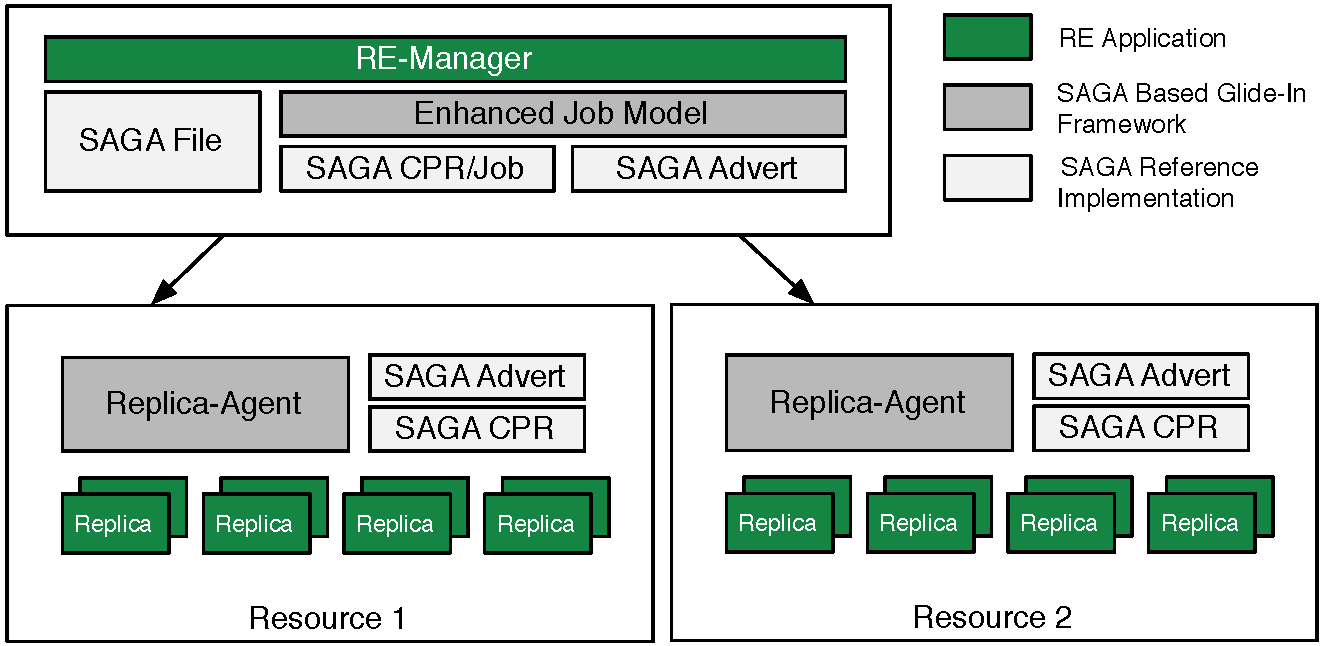
\includegraphics[width=0.9\textwidth]{remdmanager_v11}
    \caption{\footnotesize \bf The Replica-Agent is used as
      place-holder job for all replica sub-jobs running on a single
      cluster. The \remanager\ can control both the \replicaagent\ and
      the replica jobs using a SAGA-based user-level job API. By using
      this efficient way to allocate resources, queuing times are
      minimized and the time-to-completion can be dramatically
      reduced. \jhanote{AndreL: This would be a good place to
        illustrate clearly, what is a \texttt{big\_job} and 
        what is \texttt{sub\-job}}} \alnote{done.}
    \label{fig:remdmanager_v1.1}
\end{figure}

\jhanote{removed reference to programming abstraction}

\jhanote{Andre L, here is a note, which will hopefully help: as you
  know \glidein\ is a system level abstraction. So we should not say
  \glidein\ based application, but applications that use \glidein\ ,
  ie application is distinct from the system}

\jhanote{Secondly, it is important to distinguish between the new
  ``Job abstraction'' ie meta-job and simple-job as an extension of
  the SAGA job-model, from the \glidein\ abstraction. I am sure we are
  all aware of the differences, but in the writing the two seem to be
  conflated, or at least will appear conflated for a person reading
  this the first time. I would say the mata-job/simple-job is a usage
  pattern, and the \glidein\ is an abstraction that supports this
  pattern.}

\jhanote{We could probably structure the subsection on ``Efficient
  Replica Job Scheduling'' into two parts, an opening on ``Job
  Patterns and Abstractions'' and secondly
  ``Implementations''. Currently, we need more details describing
  Figure 2 and the control flow between \remanager\ and individual
  replica-jobs within a meta-job. This location of this note, is a
  good point to separate the two.}    



%\alnote{we should add some more application background (the physics behind our approach) to this paragraph}

% \alnote{TODO: Add adaptive sampling description}     
  
% The \remanager\ can rapidly execute small replica
% jobs using the enhanced Job API.
% This agent is assigned the resources required
% for all replica processes on this machine.
  
% \subsection{Implementation}         
%  
% This enhanced job abstraction is entirely implemented on user-level 
% using SAGA and Python. Using the Python duck typing mechanism the 
% \glidein\ job and sub-job object can 
% be used as drop in replacement for regular SAGA Job and CPR objects.
%                                                           
% The implementation comprises of the \glidein\ orchestrar providing the 
% enhanced job API and the Replica-Agents
% representing the place-holder jobs. When an application requests an 
% allocation of a resource chunk on a certain machine, the framework submits a
% place-holder job, the \replicaagent\ , to the respective resource
% using the SAGA CPR API. 
% 
% For every further sub-job the reference to the \replicaagent\ job id 
% is used by the \glidein\ framework to map
% the sub-job to a Replica-Agent.  For communication between the \glidein\ framework
% and the \replicaagent\ a simple protocol based on the SAGA
% Advert Service, a central key/value store, is used.  For each new job an advert
% entry is created. The \replicaagent\ periodically polls for new jobs.
% If a new job is found and resources are available, the job is launched,
% otherwise it is queued.
%            
% In a sense the resources managed by Replica-Agents can be compared to 
% a resource reservation. In principal, the Replica-Agent represents 
% a user-level resource manager for these resources. It is the responsibility 
% of the \replicaagent\ 
% to assign resources to sub-jobs and free them after completion. Further,
% the \replicaagent\ monitors all sub-jobs and registers required
% information with the Migol backend.  



% \jhanote{Let us reach consistency on, BigJob/LittleJob vs MetaJob vs
%   Enhanced Job terminology}

% resource management: how large is the glidin job?

% Further, 
% it is able to tolerate failures within the Grid infrastructure, e.\,g.\ 
% the failure of the central registry service. 

% To integrate NAMD with the SAGA/Migol infrastructure a SAGA based task
% agent -- {\it Replica-Launcher}, is used.  This agent is responsible for
% updating the metadata of the application, i.\,e.\ the state,
% monitoring endpoint and new checkpoint URLs, at the
% Migol backend.  The agent then launches the actual NAMD job using
% MPI. During the entire runtime the replica process is monitored by
% Migol using the monitoring endpoint of the Replica-Launcher. This
% Replica-Launcher enables the flexible orchestration of multiple NAMD jobs
% through the REMD-Manager without modification of the NAMD source
% itself.    This
% Replica-Launcher enables the flexible orchestration of multiple NAMD jobs
% through the REMD-Manager without modification of the NAMD source
% itself.
               
% our implementation of
% \glidein\ will then serve as a meta \glidein\, with condor level
% \glidein\ being usable where appropriate.

% thus highlighting the power of programmatic interface working on condor
% adaptor we could easily map this to condor \glidein
% {\bf This is the first known instance of creating a system
% (deployment) level abstraction from basic programming interfaces.}
 

% \jhanote{May want to replace or remove: At the same time, SAGA allows
%   the application to easily utilise other infrastructures in
%   conjunction to or as replacement to Migol.}

% \jhanote{We need to reference the challenges outlined in the previous
%   section explicitly and mention how we have addressed them}


% agile-execution that supports adaptivity, perform better than a rigid
% co-allocation scheme.
% In general, an implementation that is adaptive will have
% a lower time-to-completion. 

% Since the number of replica processes is fixed, the RE-Manager can
% simply determine the size of the Glide-In job by aggregating 
% the resources for all replica processes on a certain Grid machine.

% \section{Musings on Dynamic Resources, Adaptive Applications, and
%   RE Simulations}                                                                  
% Applications with many component (e.\,g.\ replicas) or stages (concurrent
% or sequential) may have time-varying resource requirements, e.g., in
% the number of processes, or the need to have lower queue waiting time,
% or enhanced time-to-solution of a sub-component. Such applications are
% referred to as dynamic application. Adaptivity is a mechanism to
% respond to dynamic changes as opposed to just ignoring the dynamic
% attributes. A single dynamic application may have possibly different
% adaptive strategies that can be used. There is a qualitative scale of
% ``dynamism''. At the one end of easiness, where the dynamism is very
% simple to predict, almost effectively make it static.  At the other
% end of the spectrum, there is the very difficult to predict dynamic
% requirements -- difficult either due to strong fluctuations, or just
% very different phases (irregular). Either way a static resource
% mapping strategy will not          

% On a slightly different note, it is important to distinguish between
% multiple ``heterogenous parameters'' versus dynamical attributes; we
% prefer to call an application dynamic when the resource requirement
% changes or the availability changes. In contrast, a static number of
% parameters have different values or for that matter even dynamic
% values (I would call that computational steering -- either manual or
% automated). In a nutshell, resources variability makes an application
% dynamic; a mechanism to respond to the change makes it adaptive.  


% We are going to show that as the number of resources available (pool)
% gets larger, the greater the advantages to point U even though point D
% becomes harder. A truly scalable agile-execution model requires
% support/strategies both U and D, for at some stage the inability to do
% D effectively will limit the returns on U. In this paper, we will
% focus on point U, and will discuss point D (in conjunction with U) in
% a later publication. 

% A relevant question is: Do BigJobs (using Glide-Ins mechanism) make it
% easier to do any of these directly?  At some level the answer is yes
% as it makes both tasks easier.  Instead of a single task, we are now
% looking at a higher-level task -- an aggregation, and in some ways it
% reduces the complexity.  In both cases, the sub-tasks are immune from
% the fluctuations of the scheduling system.  But the BigJobs that
% support Glide-In mechanism help with requirement U directly, and not
% directly with requirement D, thus a necessary but not a sufficient
% mechanism to respond to the dynamic nature of RE
% applications.
% 
% There is a need to distinguish between BigJob and Glide-In. One can
% have BigJob ie aggregated jobs, without supporting flexible
% scheduling/allocation within the BigJob ie the unit is now just a
% BigJob. But BigJob with Glide-In allows the aggregation of sub-jobs
% and provides the advantages of the aggregation without losing the unit
% to be a sub-job ie. scheduling/allocation is supported for individual
% sub-jobs. 

% RE in addition to being a good candidate for
% embarrassingly-distributed applications, are also very good candidates
% for using dynamic resource pools; Glide-Ins are a very useful
% abstraction for dynamic resources aggregation and utilisation.
% 
% There are different ways in which our simulation can respond
% to a change in the number of resources required/available:
% 
% \begin{enumerate}
% \item The {\bf number} and {\bf location} of BigJobs can adapt, and
%   everything else remains the same i.e, this leads to an increase in
%   the net number of replicas
% \item The size of a BigJob can adapt, keeping the number of BigJobs a
%   constant. Thus either the number of processes per replica will
%   change or the number of replicas per BigJob will change
% \item Within a BigJob (of fixed size), the number of processes
%   assigned to a replica can adapt (possibly keeping the number of
%   replicas the same, or determining some replicas to put into sleep
%   state)
% \item Again for a fixed BigJob size, assume the number of replicas
%   assigned to a BigJob can adapt, (possibly varying the number of
%   replicas in a BigJob)
% \end{enumerate}     

% Motivations for having an implementation of RE
% simulations that are adaptive (ie can respond to dynamic changes in
% resource requirements and availability).
% 
% {\it Scenario A:} Vary the number of processes assigned to each
% replica (?) by speeding up a job that is slowing down others
% 
% {\it Scenario B:} Vary the Number of replicas, (i) reassign Temp
% (refined/adaptive sampling) and, (ii) replicas at new (extended T)
% (enhanced dynamics)
% 
% {\it Scenario C:} Parallel replica dynamics: Just use the additional
% resources to be assigned to speed up the calculation.
% 
% Scenario (A) in turn could be met, when either changing the number of
% replicas (Approach 4) or changing the number of processors associated
% with each replica (Approach 3) or just use Approach 2 Scenario (B)
% could be met with Approach 4 or Approach 1.  

% Resource Determination (D): Interestingly the qualitative nature of
% the problem remains the same, just the number-of-degrees of freedom
% that need managing changes. For example, the strategy that needs to be
% determined to find optimal size and location of a BigJob is the same
% as that for non-aggregated jobs, ie. for example BQP enables both.
% (The determined optimal size of BigJob in turn influences the number
% of replicas in a BigJob or the size of individual replicas).   

% It is useful to contrast our approach to approach where a single
% application image is used (e.\,g.\ MPIg model). The MPIg approach
% has the advantage of being able to continue without
% checkpoint/restart after an exchange, but it is not agile, for
% example it needs co-scheduling of resources. This might be
% acceptable for very very large simulations or very long running
% simulations, but in general and on average, it is more likely that
% an implementation that is adaptive will have a lower
% time-to-completion.

% Scheduling - BS
% Another issue results from possibly different start times of the
% \replicaagent\ job at different resources.  


\section{Distributed Replica-Exchange on the TeraGrid}
\label{sec:exp}
        
To evaluate the performance of the RE-Manager several experiments have
been conducted on the TeraGrid and LONI resources. The TeraGrid
resources used are: Ranger, Abe and QueenBee (QB).  We investigated
the performance of the SAGA Glide-In mechanism and of the different
adaptivity modes.

\jhanote{the use of the term cluster should be consistent with the
  resource description :)}

% QB, which is both a LONI and a TeraGrid resource, is the largest
% LONI machine and has a peak performance of over 50 TFlops.
% Figure~\ref{fig:saga-taskfarming} gives an overview of the testbed.


% Scientific results obtained from using this infrastructure
% will be reported elsewhere.

\jhanote{define Generation?}  \alnote{added definition to introduction
  - should we define it here also?}  \jhanote{distinguish between
  replica, replica processes; or at least keep usage consistent}
\alnote{OK, hopefully use replica consistently} \jhanote{describe how
  exchange partner is chosen? remains the same?}\alnote{yes, the pairs
  remain the same. Added a sentence.}

The RE-Manager was configured to run a MD simulation with up to 16
replicas sampling a temperature range between 300 and
450\,K. Replica exchanges are carried out between pairs of replica
processes. Each run comprises of five generations respectively of 64
attempted exchanges.  A replica consists of a NAMD simulation
running for 500 time steps. Up to 24 MPI processes are used for
carrying out the NAMD run.

\begin{figure}[th]
    \centering      
        \subfloat[RE-Manager Scaling]{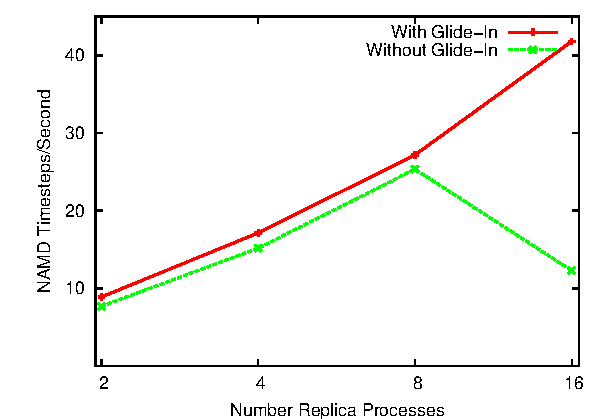
\includegraphics[width=0.48\textwidth]{performance/perf_remd_timesteps.pdf}}    
        \subfloat[Glide-In Performance]{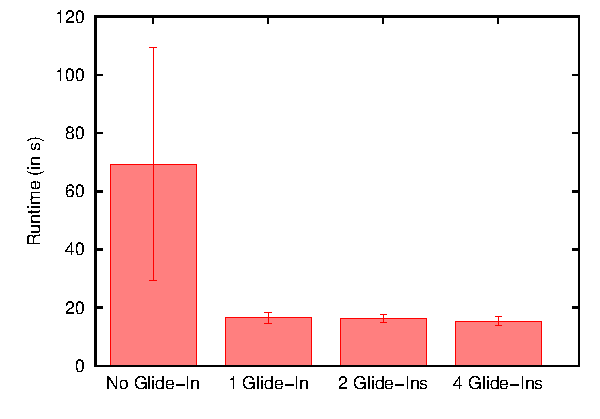
\includegraphics[width=0.48\textwidth]{performance/perf_glidein.pdf}} 
        \caption{\footnotesize \bf SAGA Glide-In and RE Performance
          (QueenBee): \jhanote{For the redline, is there just one
            glide-in that is being used, or multipled? I think the
            answer is one, but need explicit mentioning.} 
          Obviously,
          the increase in the number of resources allows sampling of a
          wider parameter range. Especially beneficial in particular
          for runs with many replicas is the clustering of
          processes using the SAGA Glide-Ins. Using a single Glide-In
          job for all replicas we observed significant performance 
          improvements of up to 80\,\%.
          \jhanote{How many
            replicas in each glide-in? In the case where there are is
            no Glide-In?}}     
           \alnote{All Replicas are within the single Glide-In, i.e. 2, 4, 8 resp. 16 replicas.
           With 0 Glide-Ins each job is separately started - no glidein is used.}
    \label{fig:perf_remd_glidin}
\end{figure} 

\subsection{SAGA Glide-In Performance}

Initially, we investigate the performance of the Glide-In framework,
which is important to support the the advanced adaptivity features of
the RE-Manager.  We compare the performance, i.\,e.\ the simulated
problem set and the runtime, of different REMD runs with and without
SAGA Glide-In on a single machine (QueenBee).
Figure~\ref{fig:perf_remd_glidin} illustrates the results.

Obviously, the increase in the number of replicas allows the
computation of a greater problem set, i.\,e.\ the sampling of a wider
parameter range (Figure~\ref{fig:perf_remd_glidin}a).  \jhanote{Once
  again, it is not obvious if the number of Glide-Ins is being
  increased on one machine?}  \alnote{I hope this becomes clear now
  with the new introduction section.}  However, the figure also shows
the limitations of the regular job submission mechanism: The more
processes are spawned, the more likely queueing delays will be.  With
the SAGA Glide-In framework the number of NAMD steps almost scales
linearly; in contrast, without SAGA Glide-In the NAMD steps metric
\jhanote{not sure what computed  problem set is...?} 
\alnote{should refer to NAMD step/s. replaced it.}
rapidly drops when using more than eight
replicas. This slowdown is caused by the delay of some replicas.  For
example, on QB we were only able to run 12 of the 16 jobs in parallel.
The remaining four replicas had to wait in the queue and produced a
significant slowdown during the synchronization after each generation.
This behaviour particularly occurs on crowded resources or if policies
at the local resource manager restrict the number of resources that
are concurrently allocated to a user.

\jhanote{unfortunately this paragraph and the one before are unclear}
\jhanote{I would recommend using time-to-completion over
  time-to-solution; also maybe use shorthand T\_c?}  \jhanote{Ah, OK
  single-machine is mentioned here now. Need to mention explicitly
  upfront} \alnote{hopefully mentioned sufficiently often now}

Figure~\ref{fig:perf_remd_glidin}b shows the effect of the SAGA
Glide-In framework on the time-to-completion ($T_{c}$) using 16
replicas on QB.  With the Glide-In framework, we were able to reduce
$T_{c}$ from 70\,minutes to about 17 minutes, which corresponds to a
decrease of about 70\,\% runtime.  In single scenarios even greater
improvements of up to 80\,\% have been observed. As described, this
effect is mainly attributed to the elimination of queuing times for
every sub-job. Once the Replica-Agent become active, replicas can be
efficiently dispatched without requiring interactions with the local
scheduler.

\jhanote{need to clarify what the 80\% means/implies?} \alnote{I refined the above
paragraph. Are there any particular implications you refer to?}

The unpredictable nature of these queueing times is reflected in the
high standard deviation observed. While long queueing times also apply
to Glide-Ins, the impact is in general less severe.  In the Glide-In
scenario, the queueing times become negligible, the longer the RE
simulation is (the runtimes have been kept short for this simple
scenario).

% In contrast, when no Glide-Ins are used every sub-jobs is subject to
% the queuing delay at the local scheduler.
In certain situations the usage of smaller jobs can have an advantage,
e.\,g.\ when the local scheduler backfills such jobs. However, usually
not all replicas can be backfilled. Also, some resources
impose a restriction on the number of active jobs per user. 

% In general, the more processes are spawned the more likely are
% delays.

The Glide-In framework represents an essential building block for
conducting efficient RE simulations. In the following,
different adaptive resource utilization schemes, which have been
implemented on top of SAGA Glide-In, are evaluated.

\subsection{Adaptive Resource Utilization}

To evaluate the different adaptive strategies, the RE-Manager
has been deployed on multiple resources  on the
TeraGrid. In particular, we investigate the effect of 
the dynamic adaptation of the \emph{replica size} (scenario A), i.\,e.\ 
the number of MPI processes assigned to each replica,  
and of the \emph{replica number} (scenario B), i.\,e.\
the number of replicas participating in a generation.  
We compare the runtime of a REMD simulation with 64 attempted 
exchanges on different sets of distributed resources and Glide-In 
configurations.  
                    
\begin{figure}[h]
  \begin{minipage}[t]{.48\textwidth}
    \begin{center}  
      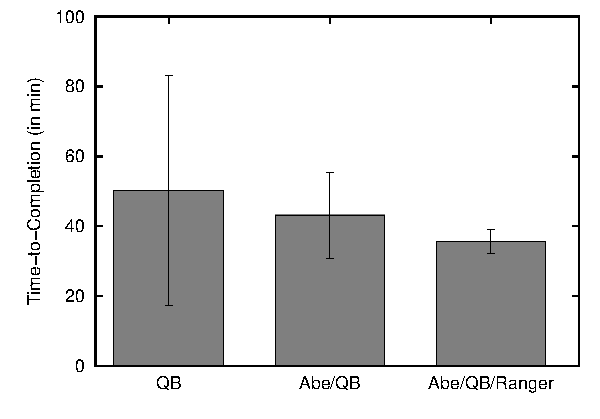
\includegraphics[width=\textwidth]{performance/perf_distributed_size_replica.pdf}
      \caption{\footnotesize \bf Replica Size Adaptivity (Scenario A):
        The number of MPI processes per NAMD tasks is dynamically
        adjusted to the number of available resources. On every
        resource 4~Glide-Ins with 32 cores each are started. A
        constant number of 16 replicas is used.  The more resources
        that are available, the more cores can be assigned to each
        NAMD task, which leads to a reduction of $T_{c}$.  }
      \label{fig:performance_perf_distributed_A}
    \end{center}
  \end{minipage}
  \hfill
  \begin{minipage}[t]{.485\textwidth}
    \begin{center}  
      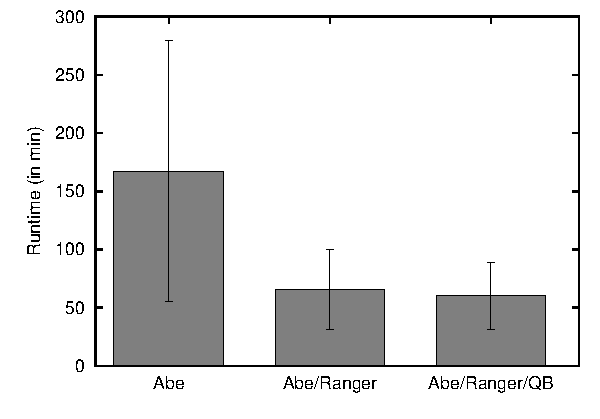
\includegraphics[width=\textwidth]{performance/perf_distributed_number_replica.pdf}
      \caption{\footnotesize \bf Replica Number Adaptivity (Scenario
        B): This scenario utilises the capability of the underlying
        physics model to dynamically adjust the number of replicas.  A
        constant number of 4 Glide-Ins with 64 cores each distributed
        across 1, 2 and 3 machines is used.  The more distributed
        resources that can be utilised, the smaller $T_{c}$.}
      \label{fig:performance_perf_distributed_B}
    \end{center}
  \end{minipage}
  \hfill
\end{figure}

% \begin{figure}[t]
%     \centering                     
%     %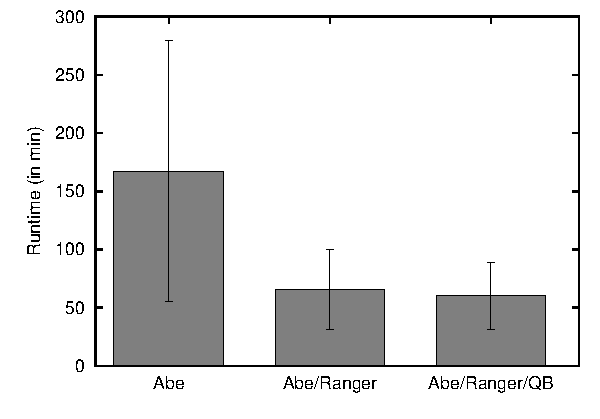
\includegraphics[width=0.48\textwidth]{performance/perf_distributed_number_replica.pdf}
%        \subfloat[Replica Process Size Adaptivity]{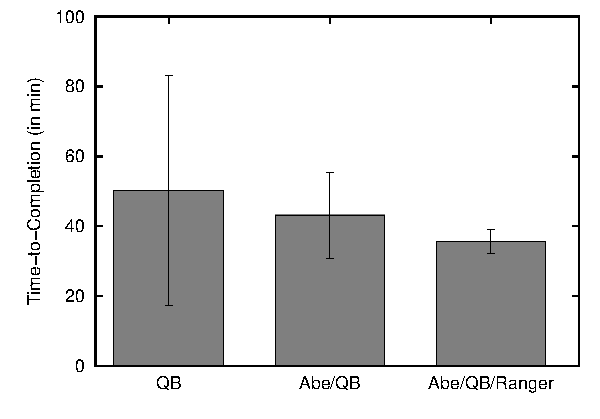
\includegraphics[width=0.48\textwidth]{performance/perf_distributed_size_replica.pdf}}
%        \subfloat[Replica Process Number Adaptivity]{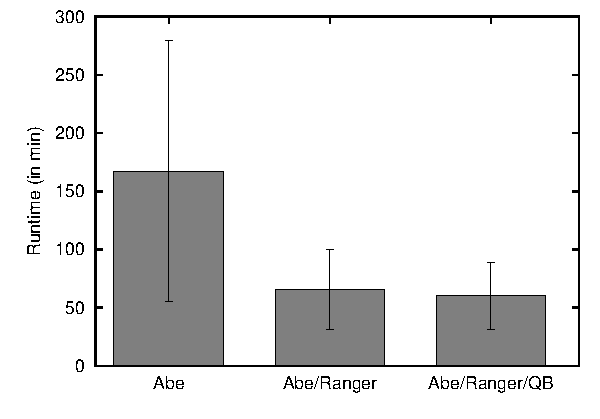
\includegraphics[width=0.48\textwidth]{performance/perf_distributed_number_replica.pdf}}    
%        \caption{\footnotesize \bf Performance of the RE-Manager: 
%          In scenario A, the size of all replica processes is dynamically adjusted to
%          the number of available resources. All resources, i.\,e.\ Ab
%          The figure shows the runtime of the RE-Manager for
%          64 pair-wise exchanges using 16 replica processes with 16
%          cores each. For all three scenarios 4 Glide-Ins with the size
%          of 64 cores are used. The utilization of more machines leads to a
%          shorter time-to-completion ($T_{c}$).          
%          \jhanote{It is not clear to me from
%            the caption whether the number of BigJobs remains the same
%            for the three scenarios presented, i.e., the difference is
%            location. Needs clarification} }
%            \alnote{The issue I have currently is that the GlideIn size and the queueing delays
%            are different between both experiments, which explains the difference in particular
%            on a single machine. }
%     \label{fig:performance_perf_distributed}
% \end{figure}   
                     
In scenario A, up to 3 resources running 4 Glide-Ins with a constant
size of 32 cores each are used, i.\,e.\ if all resources (Abe, QB and Ranger) are
available a total of 384 cores can be consumed.  During the run the
number of MPI processes for each replica is dynamically adjusted as
additional resources become available. Depending on the number of
available resources, between 8 and 24 cores are used for each replica.

\jhanote{AndreL: We need to mention explicitly that i) the size of a
  glide-in job was kept constant at 32 cores, and ii) this number of 32
  is a seat-of-the-pants/empirically derived number.}

\alnote{It is rather an intuitive number to force a lower number of
  cores per replica for the 1 resource case. Otherwise, there would
  probably no speedup for this scenario with only 500 NAMD
  steps. There is some overhead for moving replicas from one machine
  to another one (file staging).}
Figure~\ref{fig:performance_perf_distributed_A} shows the results of
the distributed run. Despite the overhead for migrating replicas to
newly available resources, a notable speedup of up to 15\,minutes can
be observed with the increase of the number of resources. However, the
measured efficiency is only about 0.5. But, this is rather a
limitation of the used setup than a general scalability barrier.  The
setup comprises of rather short NAMD jobs; in particular during the
initial phase jobs are often migrated to other resources, which mainly
causes this overhead. During longer runs resources fluctuate less
making this overhead negligible.  \jhanote{I think we need to address
  the following else we will get dinged by the referees: We increase
  our resource pool by a factor of 3, but get only a 33\% improvement
  at best} \alnote{I tried to explain this number a little better
  using the calculated efficiency: (t(1)/t(n))/n: E(2) = 0.58; E(3) =
  0.47; There are still some issues with scenario A (in particular I
  am referring to the heterogeneous speeds of these three machines
  making this increasing number of MPI processes less efficient!)}

The capability of the RE-Manager to adaptively adjust the number of
replicas simulated -- in effect adjusting the either the range of
temperature or the specific temperatures simulated, is demonstrated in
scenario B. For this purpose, 4 Glide-Ins with 64 cores each are
distributed across 1, 2 and 3 different distributed resources. That
means that the total of 256 cores is allocated on (i) Abe only, (ii)
Abe and Ranger respectively (iii) Abe, Ranger and QB.
\jhanote{AndreL: Make it easy for the ready to grasp the number of
  cores used when just Abe; when Abe/Ranger and finally when
  Abe/Ranger/QB. (i) Is it 4 glide-ins in each of the three scenarios?
  4 glide-ins on Abe, then 4 glides-in on Abe/Ranger and then 4
  glide-ins on Abe/QB/Ranger??}  \alnote{Added sentence. Answer to
  your question: yes} Each replica is started with a constant number
of 16 MPI processes.  Using adaptive temperature sampling, the number
of replicas is dynamically increased (up to 16) as the number of
available resources increases.
% A maximum of 16 replicas and 256 cores are used.

As shown in Figure~\ref{fig:performance_perf_distributed_B}, $T_{c}$
decreases with the number of TeraGrid resources used.  With the
distribution of the simulation onto multiple resources the probability
that a single heavily-utilised resource delays the overall progress of
the simulation is reduced.
% This is also reflected in the standard deviation,
% which clearly decreases as the number of distributed resources used
% increases. 
The results clearly demonstrate the benefits of the adaptive replica
scheme -- it is favourable to instantly use resources as they become
active instead of waiting for the complete set of nodes to become
available.


\jhanote{Once again, we will need to provide efficiency numbers as
  people are accustomed to seeing in parallel computing: ie
  Time-to-completion for net number of processors employed.  The point
  here is not to be defensive compared to a 100\% scaling, but the
  point is to remind that we are solving a very different problem!}
\alnote{since the number of used resources remains the same (they are just differently distributed),
the efficiency for scenario B is 1:1 reflection in the time-to-completion.}  

% This was the optimal Glide-In size
% determined in earlier experiments.  
% We measured the runtime for 64 attempted pair-wise exchanges 
% with respect to the number of TeraGrid
% resources utilised.  
\jhanote{This is going to sound bizarre... but in future we should
  probably use a power-of-two number of exchanges and not nice numbers
  like 40 or 42 :)}           
\alnote{updated it to 64... will attempt more once I have this stuff working}

% This is in particular useful for smaller resources, such as Oliver, where it 
% is only possible to request 64 cores at a time. In contrast to the QB only run, 
% the runtime only slightly increases by about 1.5 minutes, which is 
% acceptable compared to a possible delay due to insufficient resources on Poseidon.
                                              
\alnote{Unfortunately, we have not been able to replica the
  experiments without the Glide-In mechanism due to various reasons:
  MPI/Globus not correctly configured on Ranger}


\section{Related Work}

\jhanote{This paragraph discussing different Glide-In mechanisms and
  implementations needs to be moved to another section. Maybe into
  ``Related Work'', but definitely not here; it disrupts the flow.}
\alnote{ok, moved this to related work added comment why our approach is unique}

\jhanote{This section should focus on both just the ``algorithmic''
  advances/modification around Replica Exchange. But also
  advances/related work around  implementation in distributed
  environments}
                       
\alnote{Should we add related work with respect to glide-in?}

\jhanote{We should talk about Condor's glide-in, but are there other
  systems that implement glide-in features? Not that I'm aware of}

\jhanote{Joohyun: can you put in information on the AREMD and other
  papers you have sent around?}


% \jhanote{This might have to be commented out: Checkpointing and
%   rollback recovery is widely used in Grids. For example, the
%   Condor/PGRADE system~\citep{DBLP:conf/eagc/KovacsK04} consists of a
%   checkpointing mechanism for PVM applications and uses
%   Condor-G~\citep{citeulike:291860} for scheduling.  While PGRADE
%   emphasises an integrated user-level checkpoint approach, we believe
%   that this approach is not suitable for a heterogeneous Grid
%   landscape. Further, the framework does not ensure the
%   fault-tolerance of the service infrastructure sufficiently.}
                                 
\jhanote{This will have to be commented out: Further, these frameworks
  or schedulers focus on individual aspects, e.\,g.\ Nimrod-G focuses
  on task farming or GridWay on meta-scheduling. Migol aims to provide
  an overall autonomic, self-healing infrastructure, which addresses
  the fault tolerance of Grid applications and the infrastructure
  itself.}

% \noindent{\it Previous CPR Efforts:} Several frameworks for
% high-throughput computing and task farming exist,
% Condor-G~\citep{citeulike:291860}, Nimrod-G~\citep{buyya00nimrodg}, and
% Legion~\citep{689541} to name a few. These provide basic fault
% tolerance support by automatic re-scheduling failed tasks. Advanced
% features such as the management of checkpoints however, are not
% supported. Further, these frameworks rely on a very simple failure
% detection mechanism -- usually by simply polling the job state at the
% Globus gatekeeper. This allows the detection of some errors, but
% application-level failure detectors as used by the Migol/SAGA library
% can detect much more complex errors. For example, especially parallel
% applications can fail quite inconsistently: in the best case the
% application aborts, at worst the application hangs indefinitely. These
% kind of failures are not visible at Grid resource management system
% level.

% At the level of related application programming interfaces for
% checkpointing, proprietary interfaces are dominant. This is because
% applications most often rely on application level checkpointing, and
% perform also their own checkpoint management (checkpointing policies,
% frequencies, dependencies, staging etc).  \alnote{Should we remove
%   this from here - this is already mentioned now at the beginning.}
% The Open Grid Forum's\footnote{\texttt{http://www.ogf.org}} GridCPR
% group (Grid CheckPoint and Recovery) made an early attempt to describe
% a generic CPR architecture, and to define a generic CPR API, which
% would support applications to manage their complete
% checkpoint/recovery life cycle~\citep{ogf_cpr_arch}.  Based on that
% architecture, and on a set of CPR use cases~\citep{ogf_cpr_uc}, the
% SAGA group in OGF defined the CPR API package~\citep{saga_cpr_draft}
% (work in progress), whose implementation is described in this paper.
% The rendering of the CPR API in the SAGA API framework allows (a) to
% seamlessly combine CPR operations and other high level Grid
% programming abstractions provided by SAGA, and (b) to abstract from
% the actual implementation of the CPR mechanism.  The CPR API which has
% been demonstrated with the Migol framework, can work as well with
% other systems, e.\,g.\, the XtreemOS system level checkpointing
% capabilities~\citep{xtreemos_cpr}.

\noindent{\it Other Distributed RE simulations:}
Several projects, such as Folding@home and WISDOM, utilise distributed
infrastructures. While
Folding@home~\citep{PhysRevLett.86.4983}\jhanote{Folding@Home~\citep{PhysRevLett.86.4983}
is parallel replica dynamics but that is a special case of
RE; when a certain event happens, there is a need for
coordination amongst ALL replicas. We should maybe point this out,
but I think it is fair at this level of detail, to consider
folding@Home to be in the same application class to effectively
parallelize simulations} is based on BOINC~\citep{1033223}, the
WISDOM~\citep{wisdom} project utilises the EGEE infrastructure. 
Although WISDOM has similar application characteristics as discussed
here, the project is currently tied to the gLite~\citep{glite}
middleware.  In contrast to WISDOM and Folding@home, our approach is
not restricted to a specific distributed environment. SAGA based
job-launching and file-handling is supported on most general-purpose
Grids via the appropriate adaptors, as SAGA is a community
specification and is soon to be standard~\citep{saga_url}.       

LAMMPS~\citep{Plimpton:1995nx,repex_mpig} supports distributed molecular
dynamics based on MPIg~\citep{Toonen:2008ao}, which allows the
development of topology aware applications. However, this approach has
different disadvantages: 1) It represents a rather specific solution
and is less general than our RE framework. 2) LAMMPS and MPIg require
the rigid co-allocation of all resources, i.\,e.\ they may waste resources
by requiring nodes to remain idle until all resources became
available.  In contrast, our RE framework is able to adaptively use
resources as they become available.    

\cite{Woods:2005nx} deployed a RE framework on top of Condor. 
To address adaptivity the framework proposes so called catchup clusters,
which are used to speedup slow replicas. In contrast, our RE 
framework is generic and allows the utilisation of different distributed 
infrastructures (including Condor in the future). Further, it can support 
similar catchup strategies, e.\,g.\ by initially setting
the replica size  to 1; during the simulations additional resources 
can then dynamically added to slow replicas.

\noindent{\it Other Glide-In Frameworks:}   
Different systems that use similar Glide-In approaches have been
developed. \citet{citeulike:291860} initially proposed this idea in
their work on Condor Glide-In. Using Condor Glide-In a complete Condor
pool can be initiated using the GRAM service. Falkon~\citep{1362680}
is a newer system, which emphasize in particular the performance of
its task dispatcher.  However, both systems have limitations and
impose e.\,g.\ different overheads: Condor \glidein\ requires the
start of a complete set of Condor daemons within the allocated set of
resources. 
%For Falkon, \citet{citeulike:3169002}  startup time
%of over 2 minutes on a Blue Gene/P machine have been reported. 
Falkon  does not support MPI applications, i.\,e.\ it is not usable for our
application scenario.  

\jhanote{We need to mention the work using ``Catch-Up'' clusters which
  uses single processor NAMD simulations. Mention that our approach
  can effectively replicate the catch-up cluster mechanism; set all
  replica-sizes to be 1 to begin with, then those that slowdown can
  be enhanced}
\alnote{done}
% Further, firewall issues
% have been reported for both systems.

% \alnote{Should we add some details regarding the scientific results of
%   WISDOM and Folding@home and how they differ from our REMD with NAMD?
%   Or are we just comparing the Grid infrastructure?}  \jhanote{In
%   response to immediately preceeding alnote, IMHO we don't need to
%   address scientific results, but will just say the ``size of the
%   problem'' that can be studied is limited}

%% ----------------------------------------------------------------------------
\section{Conclusion and Future Work}

\jhanote{Mention BQP and co-scheduling as opposed to opportunistic
  approach. Reference Kalman-filter work. Reference Promita's work
  using BQP for tightly-coupled applications.} 
                
\alnote{I removed some parts due to redundancy}
% The RE framework uses the distributed programming
% interfaces provided by SAGA as well as the Migol middleware.  
% SAGA provides a middleware-independent, programming abstraction for distributed
% environments. With the new SAGA-CPR API RE simulations can interface
% with a checkpoint-recovery infrastructure, such as Migol. Using Migol, 
% the RE framework is able to transparently handle the failure of a Globus 
% GRAM service, a Replica-Agent or the Replica-Manager.
% 
% Using standard programmatic abstractions we have developed a general
% purpose, fault-tolerant framework that implements a commonly occurring
% application usage pattern: the loose coupling of multiple tightly-coupled
% applications. The framework is general purpose and extensible to
% different usage patterns, deployment scenarios and specific simulation
% codes. We demonstrated the successful usage of the framework to implement 
% RE simulations and to deploy these in a production Grid environment.
% 
% In contrast to other RE implementations on distributed simulations, it
% is critical to note and emphasise the general usability and
% extensibility -- across different infrastructures, across a range of
% scientific applications and usage patterns (e.g.  the multiple
% variants of the RE) -- of our approach. 


% Using the
% newly developed SAGA adaptor for Migol, any SAGA application can
% re-use Migol's fault-tolerant services for monitoring and recovery.

% The application developer is not required to provide any special code,
% just the Migol adaptor must be configured.  % The Migol framework has
% strong self-healing capabilities: critical services, such as the
% Application Information Service (AIS) are able to automatically detect
% failures and reconfigure themselves, and thus addresses common failure
% modes in distributed environments without user interaction.
% In case of failures, e.\,g.,\ a node-crash, applications are
% automatically restarted from the last saved
% checkpoint.

                    
\alnote{Attempt to structure conclusion:
1) SAGA/Migol 2.) Glide-In 3.) Adaptive Sampling 4.) Future Work: Glide-In, REMD, Reservation, BQP}
                                         
\jhanote{needs smoothening} In summary, SAGA provides a well-defined abstraction 
and Migol the underlying Grid middleware for developing and running
RE applications.
SAGA allows the simple decoupling of the RE orchestration 
logic from the underlying distributed infrastructure. All this whilst remaining
general purpose and extensible. 
Using SAGA CPR, the framework is able to utilise the Migol infrastructure, 
i.\,e. the application can benefit from features, such as the automatic 
monitoring and the transparent recovery of failed tasks.  
                 
\alnote{I used BigJob now as abstraction name...}
By only slightly extending the job model defined by SAGA, the BigJob 
abstraction could be supported and deployed within the RE framework.  
% While the current implementation of the framework uses 
% a custom protocol to implement this abstraction, it can also be applied 
% to other middleware platforms, such as Condor Glide-In.     
Based on the BigJob abstraction different adaptivity strategies for
supporting the agile execution of RE simulations in dynamic
environments have been developed. Using these strategies, the
application can agilely make use of available resources adjusting the
simulation space, i.\,e.\ the number of replicas respectively the
number of MPI processes per replica, dynamically.  With this approach
expensive idle time due to a rigid co-allocation scheme can be
avoided, which significantly reduced the time-to-completion.  While
the implementation of this abstraction is entirely based on SAGA, a
utilization of other frameworks, such as the orignal Condor
Glide-In~\citep{citeulike:291860} or Falkon~\citep{1362680}, is
possible. Currently, we are actively working on a Condor adaptor for
SAGA, which will also support native Glide-In functionality for Condor
Jobs; our BigJob abstraction will then serve as abstraction, while the
Condor level Glide-In is used as implementation where appropriate.

The adaptive RE framework has been successfully deployed within 
the TeraGrid. 
% The SAGA Glide-In framework allows the efficient
% dispatching of replicas. Using this framework the time  
% to complete could be reduced by up to 80\,\%.                                      
Using the BigJob abstraction, RE sub-jobs could efficiently be dispatched 
reducing the time-to-completion up to 80\,\%. The use of different 
adaptivity strategies to dynamically utilise additional resources lead 
to a further reduction of the time-to-completion.




\alnote{I move this to a note:
The SAGA \glidein\ framework represents the first known instance of creating a
system (deployment) level abstraction for distributed systems from
basic programming interfaces.} 

\alnote{I would not call it deployment abstraction... If I think about
deployment I am always thinking of the pain with boost.}
\alnote{I am also not sure about the ``abstraction created from 
  programming interfaces'': 
  I mean I know many abstractions which are created based on
  programming interfaces: Any C/C++-library based on the POSIX
  interfaces, higher-level Grid services based on Globus WSRF
  framework, etc.}   


% The implementation of adaptive RE minimizes slowdowns due to synchronisation, 
% whilst making it easy to add/remove resources {\it dynamically} respecting the
% underlying phys\-ics of the problem at the same time.  
       

                                 


% Currently, we are actively
% working on a Condor adaptor for SAGA, which will also support native
% \glidein\ functionality for Condor Jobs; our enhanced job model 
% will then serve as abstraction, while the Condor level 
% \glidein\ is used as implementation where appropriate.
% \alnote{This is kind of }
   
% Various optimization, such as the prefetching of tasks or the refinement
% of the deployed adaptivity strategies, can further reduce the time-to-completion. 
        
In the future, we will refine our RE framework making it
more adaptive towards dynamic environments, e.\,g.\ by deploying  
a more asynchronous scheme as described by \citet{Gallicchio:2007yq}.
Further, we will utilise our RE framework to study real science problems,
such as the Riboswitch problem~\citep{Huang:2008xe}.     

% Further, we will refine both the infrastructure and the RE algorithm
% used.  

At the same time, we will  improve our RE infrastructure to support
further adaptive strategies for resource determination and utilisation.
While it has been shown, that resources can efficiently be allocated with
the BigJob abstraction, a mechanism for dynamic resource discovery and 
for intelligent placements of jobs will be beneficial to further 
decrease the time-to-completion. 
% Currently, replicas are 
% statically assigned to resources; a good selection algorithm that favours
% less crowded resources enhances the number of resources that the RE-Manager
% can acquire for spawning replicas. 
Various approaches for the resources determination have been proposed, e.\,g.\ batch queue 
prediction~\citep{1254939,Chakraborty:2008nx} and advance reservation-based 
schemes~\citep{Jeske:2007wj}. 
% We will evaluate these systems in conjunction
% with our adaptive framework in the future. 


% However, these approaches have been designed for long-running applications. 
% In general, the scheduling 
% overhead for short-running tasks must be kept to a minimum. However, in 
% particular for Glide-In tasks such schemas could allow a further reduction of
% the queueing time and thus the time to solution.  

\alnote{I did not mention it yet, but the SD API could be a good option to control
the resource discovery.}

% queuing delays are advance reservation.  An advance reservation commits a particular
% resource over a defined time interval from the service provide to the consumer. Advance 
% reservations allow the efficient co-allocation of resources without wasting compute cycles.


\jhanote{Still sensitive to varying load-factors ie queuing delays, 
  on different machines}

\jhanote{In future work, we need to mention that we are deploying this
  infrastructure on a real distributed system (LONI) and are using it
  to study the binding interactions of peptide-RNA (Joohyun, would you
  agree?). We will report on the specific science results obtained
  using this approach in publication TBD but most likely Phil Trans of
  Royal Soc A}

\jhanote{we should also note the challenges that arise when physical
  models get very large ie low probability of exchange, reference PNAS
  paper, and how this might possibly be alleviated using distributed
  systems ie. adaptive number of replicas can be used to increase the
  probability of exchange. We are already using a variable number of
  replicas between stages, now we say we can exploit this ``feature''
  for other advantages. At least in principle.  Joohyun, you are free
  to argue otherwise....}

\begin{acknowledgement}
  This work would not have been possible without the efforts and
  support of the wider SAGA team. Important funding for SAGA
  specification and development has been provided by the UK EPSRC
  grant number GR/D0766171/1 (via OMII).  Shantenu Jha acknowledges
  the e-Science Institute, Edinburgh for supporting the research
  theme, ``Distributed Programming Abstractions''.  We would also like
  to thank Yaakoub el-Khamra for useful discussions. This work has
  also been made possible thanks to computer resources provided by the
  TeraGrid and LONI.
\end{acknowledgement}

\bibliographystyle{kluwer}
\bibliography{saga,literatur}    
\end{document}

